\documentclass[a4paper,11pt,titlepage]{report}
\usepackage[english]{babel}
\usepackage[margin=3cm]{geometry}
\usepackage[T1]{fontenc}
\usepackage[utf8]{inputenc}
\usepackage{lmodern}
\usepackage[sorting=none]{biblatex}
\usepackage{graphicx}
\usepackage{fancyhdr}
\usepackage[textfont={small,it},labelfont=bf,labelsep=endash]{caption}
\usepackage[table]{xcolor}
\usepackage{verbatim}
\usepackage[toc,page]{appendix}
\usepackage{url}
\usepackage{amsmath}
\usepackage{multicol}	% allow multi column environemnt
\usepackage{multirow}	% allow multi row environemnt
\usepackage{float} % forced position of figures/tables etc.
\usepackage{acronym}
\usepackage{rotating}
\usepackage{titling}
\usepackage{bibcheck}
\usepackage[center]{subfigure} % make it possible to include more than one captioned figure/table in a single float
\usepackage[pdfstartview=FitH,pdfborder={0 0 0},bookmarks]{hyperref}
\usepackage{memhfixc}
\usepackage{placeins}
\usepackage{longtable} % multi-page table environment
\usepackage{tabularx}
%\usepackage[pdftex]{hyperref}
\hypersetup{colorlinks=true, linkcolor=black, citecolor=black, filecolor=black, urlcolor=black,
pdftitle={U-SPACE Critical Design Report}}


\graphicspath{{./figures/}}	% look for graphic files in the "figures" subfolder

\definecolor{tableshade}{HTML}{E8E8E8}
\linespread{1.3}

% define the page headers and footers
\fancyhead{}
\fancyhead[RE,RO]{\parbox[b]{10cm}{\raggedleft U-SPACE\\ \today}}
\fancyhead[LE,LO]{\parbox[b]{10cm}{\docreference \\ \title }}
\renewcommand{\headrulewidth}{0.4pt}
\fancyhfoffset{1cm}
\addtolength{\headheight}{1cm}
\fancyfoot{}
\fancyfoot[C]{\thepage}
\renewcommand{\footrulewidth}{0.4pt}
\newcommand{\rr}{\raggedright} % to use for force left-align in multi-row table cells
\newcommand{\tn}{\tabularnewline} % to use for making the above work :-)

\bibliography{references} % include .bib file for citations

% PLEASE FILL IN THE RELEVANT INFORMATION BELOW:
%
\def\authors{ \vspace{-1.0em}
\begin{tabbing}
Omair \textsc{Sarwar} \hspace{2.5em} \= Pedro \textsc{Cervantes} \\
Morten \textsc{Olsen} \> Jan \textsc{Sommer}
\end{tabbing}
}
\def\docversion{DRAFT}					% Possible versions are: DRAFT, REVIEW or RELEASED
\def\docreference{USPACE-FR-00}	% -00 = DRAFT,  -A1 = 1st release,  -A2 = 1st release with minor updates, -B1, = 2nd release
\def\title{Final Report}


\begin{document}

\begin{titlepage}

\begin{center}


\includegraphics[width=0.6\textwidth]{figures/logo.pdf}\\[0.75cm] 

\textsc{\large Unmanned Solar Powered Airship Concept Evaluation}\\[1cm]

\line(1,0){415}\\[1mm]
\vspace{-1.0em}
\Huge \bfseries{\title}\\[2mm] 
%\
\vspace{-1.0em}
\line(1,0){415}\\[1cm]

\begin{large}
\begin{tabular}{ll}
Document Reference No.: & \docreference\\[5mm]
Document Status: & \docversion \\[1.5cm]
\end{tabular}
\end{large}

\begin{minipage}[t]{0.49\textwidth}
\begin{flushleft} \large
\emph{Authors}\\
\vspace{-1.2em}
\line(1,0){125}\\
\footnotesize{\authors}
\end{flushleft}
\end{minipage}
\begin{minipage}[t]{0.49\textwidth}
\begin{flushright} \large
\emph{Supervisors}\\
\vspace{-1.2em}
\line(1,0){125}\\
Kjell \textsc{Lundin}\\
Alf \textsc{Wikstr\"{o}m}
\end{flushright}
\end{minipage}

\vspace{1cm}

\begin{minipage}[t]{0.49\textwidth}
\begin{flushleft} \large
\emph{Project Manager}\\
\vspace{-1.2em}
\line(1,0){125}\\
Dries \textsc{Agten}
\end{flushleft}
\end{minipage}
\begin{minipage}[t]{0.49\textwidth}
\begin{flushright} \large
\emph{Quality Manager}\\
\vspace{-1.2em}
\line(1,0){125}\\
Morten \textsc{Olsen}\\[1cm]
\end{flushright}
\end{minipage}

\vfill

\begin{large}
\today \\
Lule\r{a} University of Technology \\
Rymdcampus, Kiruna, Sweden\\
\end{large}

\end{center}

\end{titlepage}

\pagestyle{plain}
\pagenumbering{roman}

\thispagestyle{plain}
\chapter*{Normative References}
\markboth{Normative References}{Normative References}
\addcontentsline{toc}{chapter}{\protect\numberline{}Normative References}
%
\begin{table}[H]
\centering
\caption{Normative References for this document}
\label{tab:normative_references}
\begin{tabular}{lll}
\hline
\textbf{Document title} & \textbf{Doc. Ref. No.} & \textbf{Doc. status}\\
\hline
Critical Design Report & USPACE-CDR-A2 & Released\\
\hline
\end{tabular}
\end{table}
%
\newpage
%
\thispagestyle{plain}
\chapter*{Document Change Record}
\markboth{Document Change Record}{Document Change Record}
\addcontentsline{toc}{chapter}{\protect\numberline{}Document Change Record}
%
%
\begin{table}[H]
\centering
\caption{Document Change Record for this document}
\label{tab:document_change_record}
\begin{tabular}{p{0.22\textwidth}p{0.25\textwidth}p{0.42\textwidth}}
\hline
\textbf{Doc. version} & \textbf{Change date} & \textbf{Change Description}\\
\hline
USPACE-FR-A1 & \today & 1st release\\
\hline
\end{tabular}
\end{table}
\thispagestyle{plain}
\chapter*{Acronyms}
\markboth{Acronyms}{Acronyms}
\addcontentsline{toc}{chapter}{\protect\numberline{}Acronyms}

\begin{multicols}{2}
\begin{acronym}
\acro{ADCS}{Attitude determination and control}
\acro{ADC}{Analog to Digital converter}
\acro{ADS}{Attitude Determination System}
\acro{BCR}{Battery Charge Regulator}
%\acro{BJT}{Bipolar Junction Transistor}
%\acro{CC}{Constant Current}
\acro{CDR}{Critical Design Review}
%\acro{CM}{Current Mode}
\acro{COTS}{Commercial Off-The-Shelf}
\acro{CPU}{Central Processing Unit}
\acro{CRC}{Cyclic Redundancy Check}
%\acro{DCM}{Discontinuous Conduction Mode}
\acro{DM}{Development Model}
\acro{DSP}{Digital Signal Processor}
\acro{ECSS}{European Cooperation for Space Standardization}
\acro{EGSE}{Electrical Ground Support Equipment}
\acro{EKF}{Extended Kalman Filter}
\acro{EMC}{Electromagnetic Compatibility}
\acro{EMI}{Electromagnetic Interference}
\acro{EPS}{Electrical Power System}
\acro{ESC}{Electronic Speed Control}
%\acro{ESR}{Equivalent Series Resistor}
\acro{ETSI}{European Telecommunications Standards Institute}
\acro{FM}{Flight Model}
%\acro{FRR}{Flight Readiness Review}
\acro{GPS}{Global Positioning System}
\acro{$I^2C$}{Inter-Integrated Circuit}
\acro{IC}{Integrated Circuit}
%\acro{IDC}{Insulation Displacment Connector}
\acro{IRF}{Swedish Institute of Space Physics}
\acro{ISE}{Integrated software environment}
\acro{ITPU}{Imaging and Tracking Payload Unit}
\acro{ITU}{International Telecommunication Union}
\acro{LDO}{Low-dropout}
\acro{LiPo}{Lithium-Polymer}
\acro{LTU}{Lule\r{a} University of Technology}
\acro{MCC}{Motor Control and Communication}
\acro{MCU}{Micro-Controller Unit}
%\acro{MEA}{Main Error Amplifier}
\acro{MGSE}{Mechanical Ground Support Equipment}
%\acro{MOSFET}{Metal-Oxide-Semiconductor Field-Effect Transistor}
%\acro{MPP}{Maximum Power Point}
\acro{MPPT}{Maximum Power Point Tracking}
%\acro{MPPTU}{Maximum Power Point Tracking Unit}
\acro{MSE}{Mechanical Structure and Envelope}
%\acro{NTC}{Negative Temperature Coefficient}
\acro{OBDH}{Onboard Data Handling}
%\acro{OpAmp}{Operational Amplifier}
\acro{OSI}{Open Systems Interconnection}
\acro{PCB}{Printed Circuit Board}
\acro{PDR}{Preliminary Design Review}
%\acro{SA}{Solar Array}
%\acro{PSA}{Pressure Sensitive Adhesive}
%\acro{PTC}{Positive Temperature Coefficient}
\acro{PWM}{Pulse Width Modulation}
%\acro{RHPZ}{Right Half Plane Zero}
\acro{RMP}{Rounds Per Minute}
\acro{SAR}{Solar Array Regulator}
\acro{SD}{Secure Digital}
\acro{SMD}{Surface-Mount Device}
\acro{SoC}{System on Chip}
\acro{SPA}{Solar Powered Airship}
\acro{SSC}{Swedish Space Corporation}
\acro{TBD}{To Be Decided}
\acro{U-SPACE}{Unmanned Solar Powered Airship Concept Evaluation}
\acro{UART}{Universal Asynchronous Receiver/Transmitter}
%\acro{UAS}{Unmanned Aircraft System}
%\acro{UAV}{Unmanned Aerial Vehicle}
\acro{USB}{Universal Serial Bus}
\acro{UVLO}{Under-Voltage Lock-Out}
\acro{TTC}{Telemetry, Tracking and command}
\acro{ISM}{Industrial, Scientific and Medical}
\acro{RF}{Radio Frequency}
\acro{TC}{Telecommand}
\acro{TM}{Telemetry}
\acro{URL}{Uniform Resource Locator}
\end{acronym}
\end{multicols}

\markboth{List of Figures}{List of Figures}
\addcontentsline{toc}{chapter}{\protect\numberline{}List of Figures}
\listoffigures
\newpage

\markboth{List of Tables}{List of Tables}
\addcontentsline{toc}{chapter}{\protect\numberline{}List of Tables}
\listoftables
\newpage

\tableofcontents
\newpage
\acresetall	%reset acronyms which is otherwise used in list of figures or tables
\clearpage %reset page numbers
\pagenumbering{arabic}
\pagestyle{fancy}

\newpage
\section{Introduction}
\label{sec:introduction}

The \ac{EPS} provides power to motors, the on-board computer, communication system and payloads. Power is mainly supplied from solar cells but can also be supplied from a battery, when solar power is not available or insufficient. 

\subsection{Changes from PDR to CDR}
\label{sec:changes_pdr_to_cdr}
%
Table \ref{tab:pdr_to_cdr} lists major design changes from the \ac{EPS} \ac{PDR} report.

\begin{table}[H]
\centering
\caption{U-SPACE \ac{EPS} design changes from PDR to CDR}
\label{tab:pdr_to_cdr}
\begin{tabular}{p{0.25\textwidth}p{0.2\textwidth}p{0.45\textwidth}}
\hline
\textbf{Area of change} & \textbf{Changed parameter } & \textbf{Argumentation for change}\\
\hline
Total power budget & Increased to $>40\,W$ & Airship total mass and size are increased thus requiring much more power for the motors\\
Solar cells & New part & Old solar cell was much heavier than listed in manufacturer datasheet due to a glass cover\\
Total system cost & Increased to $>12000\,SEK$ & Increased power and new light-weight solar cells are more expensive\\
Solar cell mounting & New part & New solar cell is flexible instead of rigid and can be mounted with \ac{PSA}\\
\hline
\end{tabular}
\end{table} 
\newpage
\chapter{Design Changes}
\label{chap:design_changes}
% what major design changes have been introduced since the CDR report? Argument why these changes were necessary. Also, will be good to include test results (functionality, weight, performance etc.) which are not documented in the CDR report.


\section{Project Schedule, Resources and Goals}
%responsible: Morten

\section{Electrical Power Subsystem}
%responsible: Morten

\section{Mechanical Structure and Envelope}
%responsible: Pedro 

\section{Motor Control and Communication}
%responsible: Pedro and Morten

\section{Imaging and Tracking Payload Unit}
%responsible: Jan

\section{Telecommunication}
%responsible: Omair
\newpage
\chapter{Flight Test}
\label{chap:flight_test}

\section{Flight Objectives and Planning}
%write for each subsystem

For the \ac{EPS}, the main test objectives were to: 
%
\begin{itemize}
\item Test if suitable power could be supplied to the motors for steering and forward propulsion
\item Confirm plausibility of providing all power from solar cells, i.e. estimate required amount of propulsion power
\item In-flight functional test of EPS telemetry and telecommand 
\end{itemize}
%
%
\section{Flight Results}
\label{sec:flight_results}
%write for each subsystem
%
%
\begin{figure}[H]
\centering
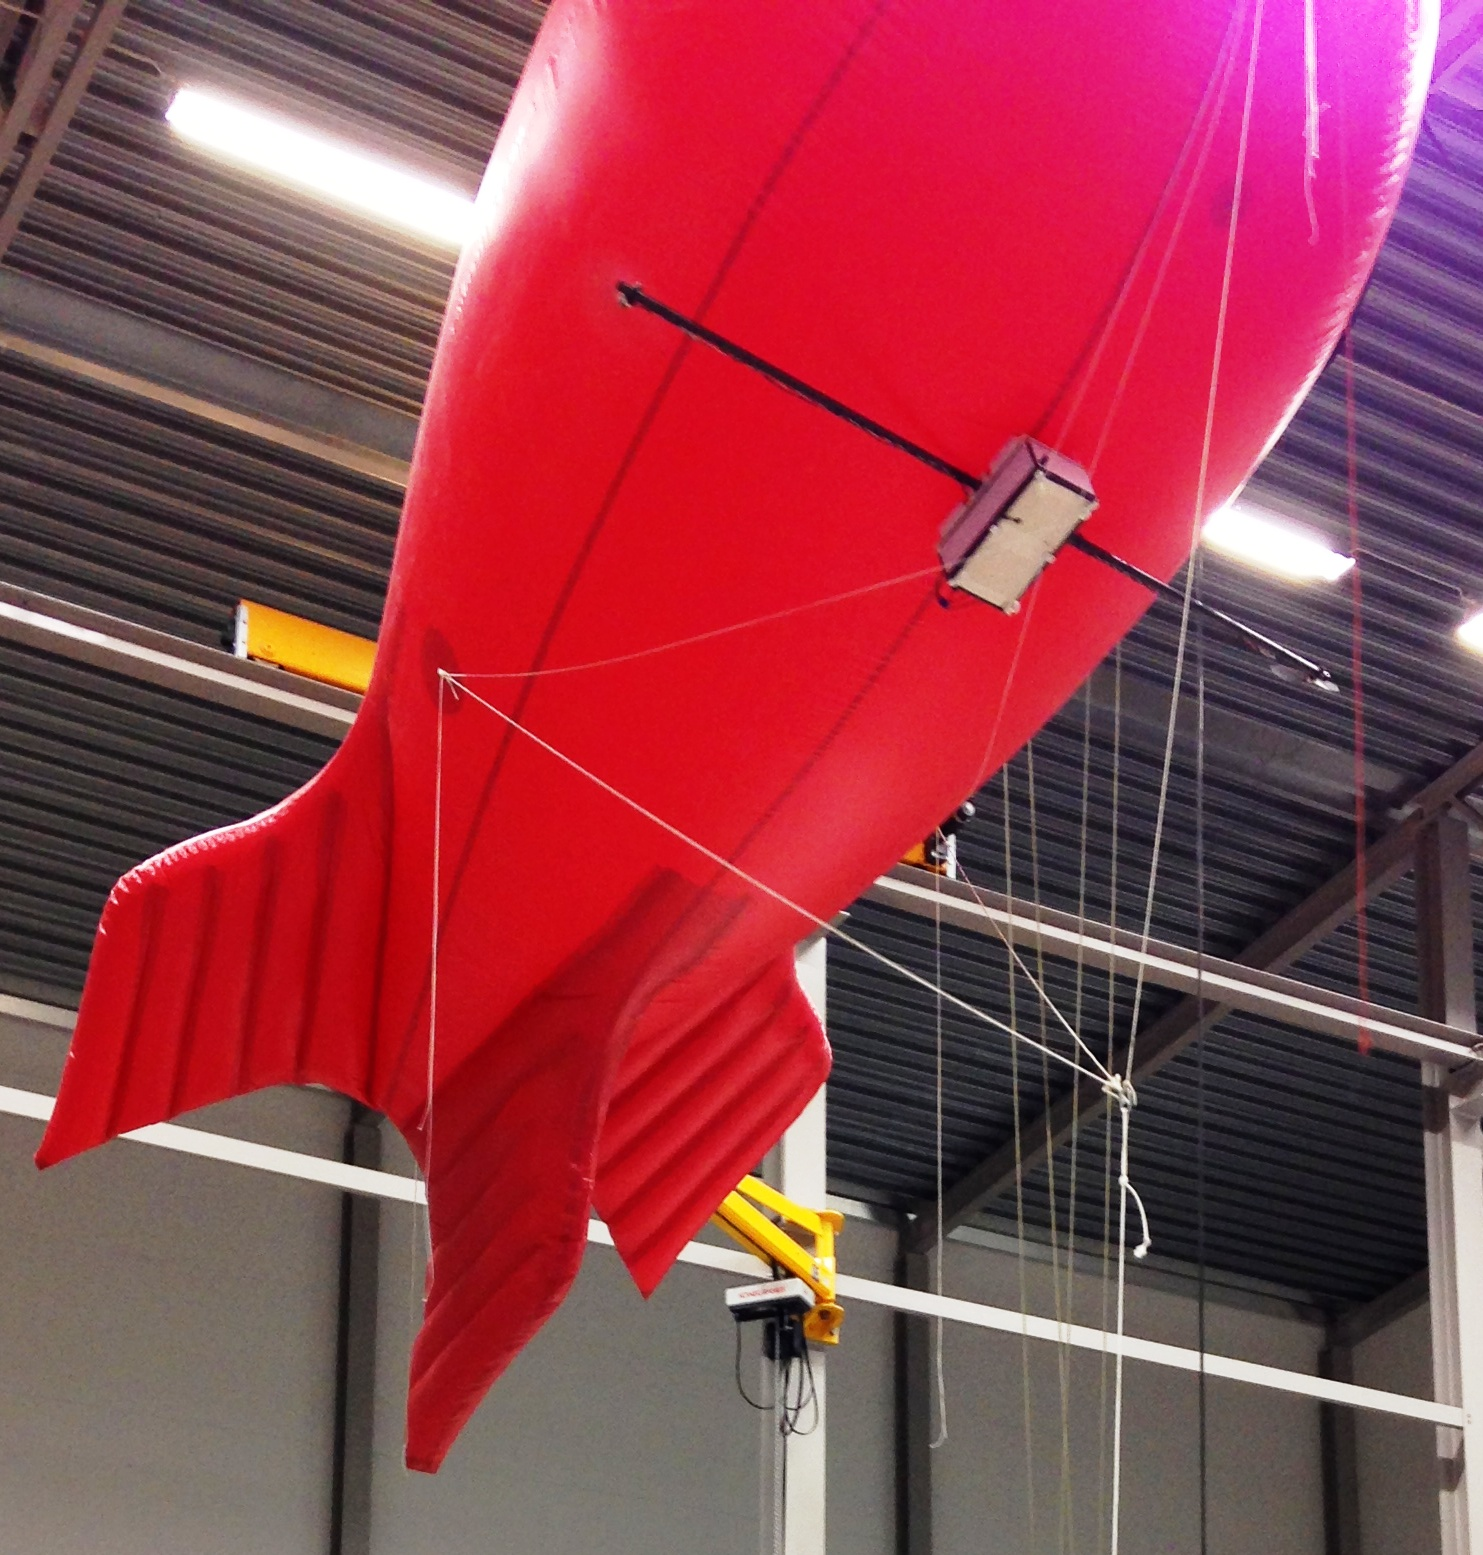
\includegraphics[width=0.7\textwidth]{figures/fig_FlightTest1_1}
\caption{First U-SPACE flight test}
\label{fig:FlightTest1_1}
\end{figure}
%
\begin{figure}[H]
\centering
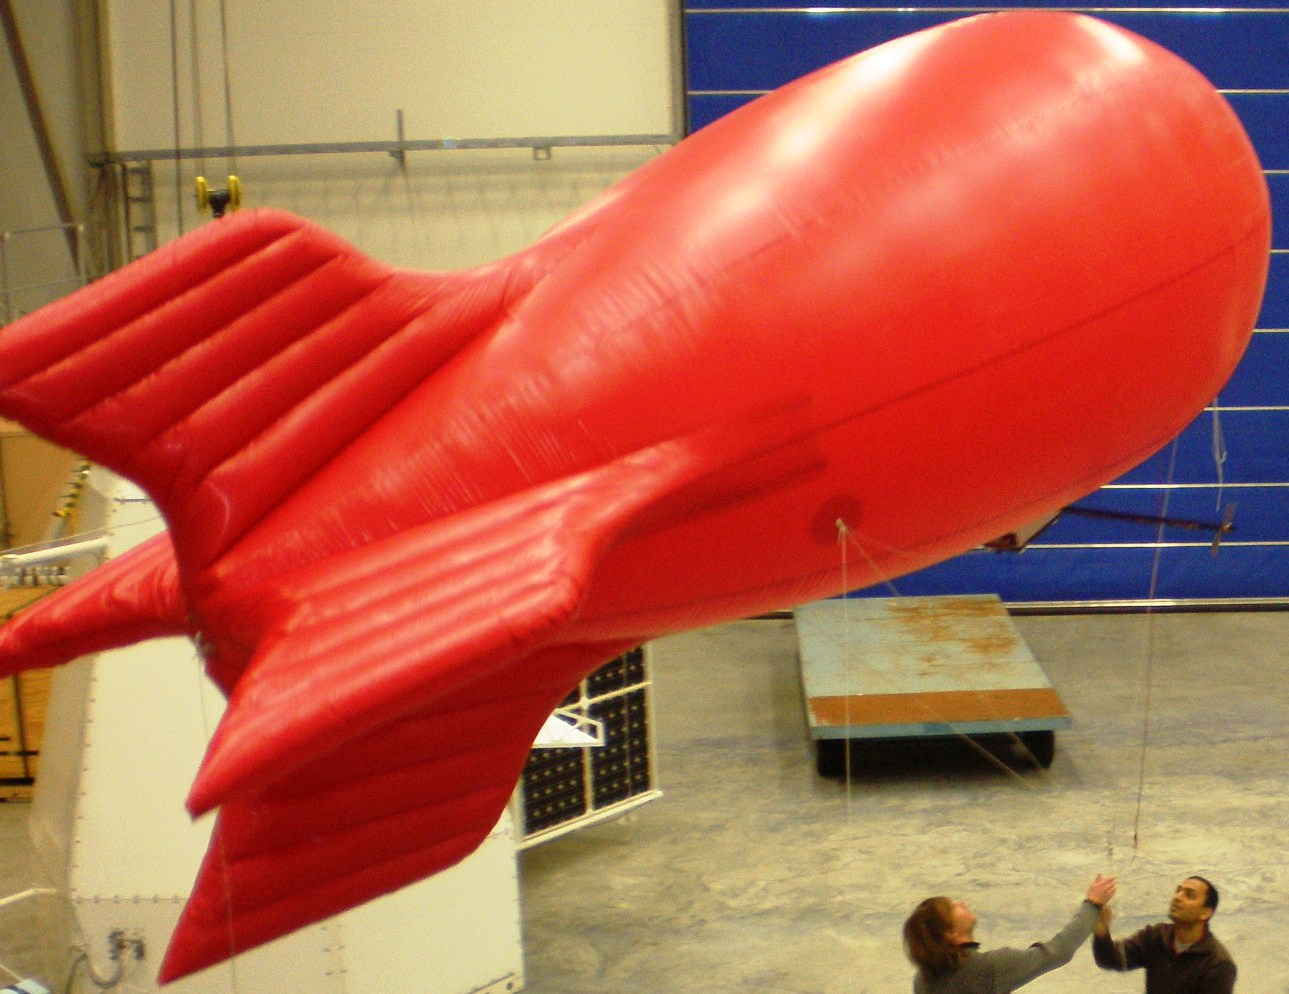
\includegraphics[width=0.7\textwidth]{figures/fig_FlightTest1_2}
\caption{First U-SPACE flight test}
\label{fig:FlightTest1_2}
\end{figure}
%
\subsection{Flight results for MCC}
At full throttle on the motors, we were able to propel the blimp forward and steer it to the side. However, it was clear that the amount of thrust generated by the motors was insufficient to properly propel the blimp. During the flight test, the blimp was attached to a concrete block on the ground via. a thin rope. When moving forward, the rope would stretch at an angle w.r.t. zenith and thus pull back the blimp. This made it difficult to estimate exactly the maximum velocity possible to obtain with the applied motor thrust. In this test, no attempt was made to "balance" out the lift of the blimp to the total mass of the U-SPACE systems. In future flights, it is recommended to balance out the lift using some dead weights (sand, small rocks etc.).


\subsection{Flight results for MSE}
%

\subsection{Flight results for ITPU}
%
Shortly before the flight test the BB failed. The attempted provisory fix using a BB-xM turned out to unstable during the flight test (see also \ref{sec:changes_itpu}). While trying to fixate cable connections between the BB-xM and the expansion board cable broke and damaged the expansion board unable to repair on the test side. Therefore the test results presented here are taken from the pre-flight test which was done in the facilities of LTU Kiruna when the original BB was still operational.
<<<<<<< HEAD
=======

\begin{figure}
\centering
\includegraphics[width=0.55\textheight]{figures/full-system-setup}
\caption{Full system setup}
\label{fig:FlightTest1_1}
\end{figure}

An image of the full system setup including all electronical moduels can be seen in figure . This setup was then mounted into the payload box (see \textcolor{red}{REF!!!}) for testing. As mentioned in section \ref{sec:changes_itpu}, operating both the ADCs of the telemetry subsystem and the sensors of the attitude determination subsystem on the same I2C-bus caused problems which needed manual reset of the I2C-bus in order to get it working again. Peculiar was that both system worked when only one of the two ADCs where connected to the I2C bus together with the attitude sensors, but failed when both ADCs were connected. As the attempts to enable a second I2C-bus on a different expansion header of the BB were unsuccessful, it was decided to test only with one ADC and in turn loose 8 of the 16 telemetry values of the internal voltages. 

With this decision implemented the testing went successful. The wireless connection to the groundstation could be established (for more see \textcolor{red}{REF TO OMAIR}). After calibration of the magnetometer, the attitude determination system was able to determine the attitude stabily and produce the roll-, pitch- and yaw-angles for the telemetry system. When receiving the corresponding signal from the communication module the camera could be activated and shoot either single images or multiple images with a set period (fastest 1~s) and save them to the onboard sd-card.  
>>>>>>> 4fb6c5e283e39b3c694310944a6c6ff9cc25aad8

\begin{figure}
\centering
\includegraphics[width=0.55\textheight]{figures/full-system-setup}
\caption{Full system setup}
\label{fig:FlightTest1_1}
\end{figure}

An image of the full system setup including all electronical moduels can be seen in figure . This setup was then mounted into the payload box (see \textcolor{red}{REF!!!}) for testing. As mentioned in section \ref{sec:changes_itpu}, operating both the ADCs of the telemetry subsystem and the sensors of the attitude determination subsystem on the same I2C-bus caused problems which needed manual reset of the I2C-bus in order to get it working again. Peculiar was that both system worked when only one of the two ADCs where connected to the I2C bus together with the attitude sensors, but failed when both ADCs were connected. As the attempts to enable a second I2C-bus on a different expansion header of the BB were unsuccessful, it was decided to test only with one ADC and in turn loose 8 of the 16 telemetry values of the internal voltages. 

With this decision implemented the testing went successful. The wireless connection to the groundstation could be established (for more see \textcolor{red}{REF TO OMAIR}). After calibration of the magnetometer, the attitude determination system was able to determine the attitude stabily and produce the roll-, pitch- and yaw-angles for the telemetry system. When receiving the corresponding signal from the communication module the camera could be activated and shoot either single images or multiple images with a set period (fastest 1~s) and save them to the onboard sd-card.  

\section{Discussions and Future Recommendations}
%write for each subsystem
%
\subsection{EPS}
Due to the connector issues discussed in section \ref{sec:flight_results}, no telemetry was available during flight, thus detailed information of power consumption were not obtained. However, at full thrust, the system has in laboratory shown to draw around 2 x 7.5 A. At a voltage of approximately 7.0 V this corresponds to 105 W power delivered to the motors. In \cite{CDR} the \ac{EPS} was designed to deliver minimum 40 W of continuous solar power. With these flight results, to allow continuous flight, future designs should increase the solar array power output by at least a factor 2.5-3.
 
The \ac{BCR} should be re-designed for higher voltage and current outputs. Options for this were discussed in section \ref{sec:changes_BCR}. This also requires a battery pack with higher voltage. An advantage with higher voltage is that the power distribution efficiency is increased, since the diode voltage-drop losses and resistive losses ($I^2 \times R$) are relatively reduced when comparing to the total amount of handled power. 
%
\subsection{MCC}
From the previous discussed flight results, it was shown that the amount of generated thrust was just barely able to move the blimp. According to \cite{website:ModelMotors}, the motors have a relatively poor efficiency of around 67\%, especially when operating at heavy loads (high currents + low \ac{RMP}). The TIF-250 blimp from Esrange has a volume of $15 m^3$ and thus an approximate lift of around 15 kg. Including the motor efficiency, the power-to-lift ratio is 4.7 W/kg. Calculating this ratio for the Zeppelins that flew during the 1930's\cite{website:graf_zeppelin} gives 15.4 W/kg for the LZ-129 Hindenburg and 19.2 W/kg for the LZ-127 Graf. Thus the U-SPACE design has a power-to-lift ratio about 3-4 times less than old commercial designs. This agrees well with the lack of motor power to properly propel the blimp. The Zeppelins were designed for a cruise speed around 125 km/h (35 m/s) which is of course faster than the U-SPACE requirement. For future designs, it is recommended to include more powerful motors designed for low speed, low \ac{RPM} and high torque like \cite{website:ModelMotors_AXI5360}. Larger motors will also require a larger solar array to provide the power.

\newpage
\chapter{Project Evaluation}
\label{chap:evaluation}
% provide feedback about the project course: what was good/fun/etc.?, what did you learn?, what didn't work well?, what can be improved for future projects?, other comments...
%This is mainly for feedback to Thomas, Kjell and LTU.

\section{Overall Project Conclusion}
%Final budget status
%What project goals were achieved?
%
The U-SPACE project has demonstrated the student design of a battery powered airship capable of forward propulsion and steering, collecting and downlink of housekeeping data as well as supporting a small scientific payload (camera). Furthermore, it confirms the plausibility of having a completely solar powered airship also when considering the extremely limited lifting mass of the blimp used for the initial test flight.
%
%
\section{Pedro}
In general I am quite satisfied with how the project course turned out. I am very satisfied with the group of people I had to work with and I think it has been a very useful experience for the future. 
However I cannot help but feeling that the coordinators of the project, i.e. whoever is in charge of the decision regarding budgets, reports, ECTS distribution and so on, did not had a well-defined protocol for this course. Because of this I think we wasted a lot of time waiting for answers that should already be clear the moment the university is offering this kind of course. The worst of all is that we wasted the entire previous summer semester because of this. Of course money is money, which is always the main issue, but after all we were a big group of people that just wanted to work. I think that if the university is offering this possibility, the process once the group has presented its ideas properly in a PDR should be a hundred times swifter in case the project is approved. 
But forgetting all the bureaucratic BS, I think the people at LTU Kiruna and IRF were always available to lend us a hand, even when sometimes it was not even their duty and that I really appreciate and I am very thankful for.
%
%
\section{Omair}
It was an interesting and challenging project for me. I learnt different tools during the project phase. These include designing a communication protocol for a wireless system, programming of an arm processor, \ac{PCB} schematic design and especially their etching in the laboratory. Beside these technical tools, I also leant documentation of a technical project which will be very fruitful for me in future projects. I learn about the different parts of aircraft/spacecraft theoretically but \ac{U-SPACE} provided me the platform to get practical experience of about every subsystems of a satellite. In short, it is a good course which helps to work independently on in the area of personal interest. 
%
\section{Jan}
%
%
\section{Morten}
In overall, the project course was personally for me a useful experience. As a quality/project manager, I experienced many of the typical challenges in project management such as time delays, rephrasing of project goals and system concepts as required, bureaucracy issues, budget constraints, changes in team structure (people leaving, people joining), challenges getting access to components and equipment/labs etc. However, it is also my personal belief that many of these problems could easily have been avoided by better communication and organization with the LTU administration at the beginning of the project. This would allow more advanced (and complete) technical systems to be developed, focusing more on the real technical challenges leading to greater project successes and providing good PR source for LTU and the students when project results are displayed in media. It is my belief that LTU has some great facilities to support very interesting student projects and they should thrive to exploit and nurture this opportunity.
%
Some personal suggestions or comments for future projects:
\begin{itemize}
\item Establishment of Viking room as permanent project room.
\item Always access to a "professional" solder station, possibly even with ESD-protected table + wrist bands.
\item Throughout the project, we were extremely dependent on Lars to get simple components/tools (resistors, wires etc.). This cost us a lot of time, whenever he was not available. If possible, a box of standard components (resistors, capacitors, simple ICs, wires etc.) should be made available to at least one person (if not all) in the project team. A simple account-sheet could be placed next to the box, where people can note what they take.
\item Quicker release of initial project budget to allow first order of components.
\item Access to workshop, once established, worked very well (except some issues with the electronic lock). This access should be established from the beginning of the project.
\item Generally we received good support from IRF, borrowing tools and suggestions for mechanical design. If possible, more instructions and recommendations from IRF experts would be helpful (soldering course, how to check solderings under microscope).
\item More critical design feedback and suggestions from supervisors, where possible, would be good.
\item More clear initial communication of project course requirement in terms of reports and presentations (how many, which and when). Ideally a document should be generated which states all specifications to the project course (budget, reports, flight-options/rules, expected support from IRF and LTU, course rules for non-EU students, course registration if done in spring semester, possibility to order components from foreign countries, etc.).
\item Project budget was not tightly maintained by students in the beginning. But also, some costs (e.g. styrofoam and possibly more) were not communicated to the group and exact amount of budget per student was very unclear throughout most of the project.
\item Especially the Spacemaster students are quite restricted in their time schedule since many of us only have half a year in Kiruna, leaving around June and the rest leaving around January/February the following year. Hence, deadlines and time restrictions stated by these project groups should be well noted and respected.
\end{itemize}
\newpage
\chapter{Future Visions}
\label{chap:visions}
% future project visions for U-SPACE
%
It is the authors's believe that designing and building an airship is a great way for students to gain initial practical experiences on project work subjected to many of the same technical constraints also found in real space projects, including:
%
\begin{itemize}
\item Very limited power budget
\item Strong mass constraints due to limited lift mass
\item Thermal constraints considering daily and seasonal weather conditions, when flying outdoors
\item System autonomy, since no physical access to systems is possible once flying in the sky
\item Support requirements for scientific payloads
\item Mechanical structure optimized for low weight with strength and rigidity to withstand non-nominal situations (uncontrolled landings etc.)
\end{itemize}
%
Airships provide low cost and frequent flight opportunities thus allowing flight experience for all students involved in the project, even if only for a single semester.  Furthermore, if means are added to reuse helium gas after flight, one of the main expenses in these systems, flight costs can be reduced to almost zero.
Due to the recent popularity of private \ac{RC}-planes, many airship components can be found at low cost and high quality such as Li-ion batteries, motors, propellers and motor controllers.
\\\\
%
\noindent
The U-SPACE project has shown the way for many possible future upgrades which can be realized in student projects, including (but not limited to): 
%
\begin{itemize}
\item Realizing a completely solar powered flight in outdoor conditions.
\item Designing and building a custom envelope optimized for low weight and mechanical properties (rigidity, mounting options, ease of manufacturing etc.)
\item Altitude control system. This could be realized by having a compressor and an air-filled envelope. When inflating the air-filled envelope, it will compress the helium envelope thus reducing the lift of the airship (same concept as used on the old Zeppelins).
\item Attitude and flight path control system. Possibility to add coordinates and positions that the airship should automatically follow or maintain.
\item System up-scaling: Higher motor power, more lift capability to support larger and more sophisticated scientific payloads.
\item Scientific payloads: Atmospheric measurements (ice crystals, meteorological etc.), simple Synthetic Aperture Radar(as demonstrated by MIT lecturer in Optics and Radar course), space elevator demonstrator,...
\item Ground link with LTU ground station. Thus providing a professional high-bandwidth communication link and a test environment for students to gain experience as ground controllers who could then also support international cubesat missions around the globe.
\end{itemize}

\newpage
\printbibliography
\markboth{Bibliography}{Bibliography}
\addcontentsline{toc}{chapter}{\protect\numberline{}References}
\newgeometry{margin=1.5cm}
\pagestyle{plain}

%\appendix

\chapter{Some Appendix}\label{app:SomeAppendix}
some text...

\chapter{Another Appendix}\label{app:AnotherAppendix}
some text...

\end{document}